\documentclass[a4paper,10pt]{article}
\usepackage[english]{babel}           % LANGEUAGE, UTF-8
\usepackage[utf8]{inputenc}
\usepackage[T1]{fontenc}
\usepackage{url}                      % Url
\usepackage{listing}                  % Code block library
\usepackage{algpseudocode}            % Pseudocode library
\usepackage{algorithm}                % Algorithms
\usepackage{amsmath}                  % ALL MATH FEATURES
\usepackage{graphicx}                 % GRAPHICS                  
\usepackage{float}                    % IMPROVED FIGURE POSITIONING
\usepackage[labelsep=period]{caption} % IMPROVED CAPTIONS
\usepackage{url}                      % WRITE URLS
\usepackage{tikz}                     % MAKE TIKZ VECTOR GRAPHICS
\usepackage{tocloft}                  % CONTROL TABLE OF CONTENTS
\usepackage[authoryear,round]{natbib} % REFERENCES
\usepackage{apalike}

%opening
\title{Population reducer}
\author{Otto Hannuksela}

\begin{document}

\maketitle

\section{Brief description of the code}

The population reducer is meant for separating different populations within velocity distributions from each other. The aim of the code is to provide a way to analyze different populations 
in a robust way. For example, it might be important for the user to be able to separate backstreaming populations from core maxwellian populations.


\section{Algorithm employed}

\subsection{Short description}

The algorithm relies on locating \emph{local maximas} within the velocity distributions. The idea is that we assume each velocity population has a local maximum somewhere, and that 
different populations are connected by a local minimum:

\begin{figure}[H]
 \centering
 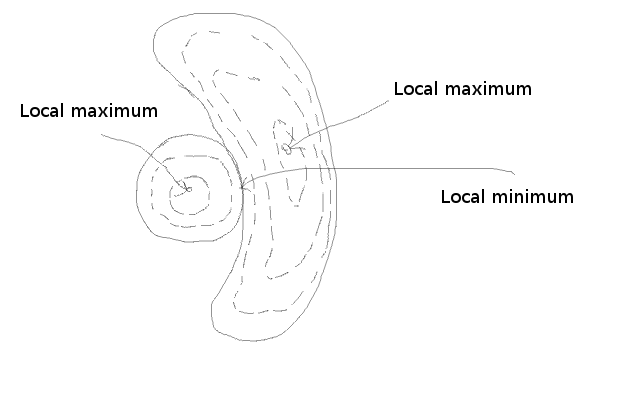
\includegraphics[width=\textwidth]{reducepopulation.png}
 \label{fig:populationcode}
\end{figure}


In this case we can assume that by iterating through velocity space starting from the largest value and moving to the next-largest value on every iteration, we finally hit the local minimum 
shown in Figure \ref{fig:populationcode}, and get two separate populations.

\subsection{Pseudocode}

\begin{algorithm}
 \label{pseudo:population}
 \caption{Population algorithm}
\begin{algorithmic}[1]
 \Function{Population\_reducer}{$cell$, tolerance}
  \State $vcells \gets get\_velocity\_cells(cell)$
  \State $sort(vcells)$ based on their value
  \State Let $populations$ be all populations
  \For{ all velocity cells $vcell$ in $vcells$ }
   \If{$vcell$ neighbor of any $population$ in $populations$}
    \If{$vcell$ neighbor of one $population$}
     \State $population \gets vcell$
    \ElsIf{$vcell$ neighbor of more than one $population$ in $populations$}
     \State Let the populations be $population1$, $population2$
     \If{$population1$ or $population2$ small}
      \State $Merge(population1, population2)$
     \Else
      \State $population1 \gets vcell$
     \EndIf
    \EndIf
   \Else
    \State $population \gets new\_population()$
    \State $population \gets vcell$
    \State $populations \gets population$
   \EndIf
  \EndFor
 \EndFunction
\end{algorithmic}
\end{algorithm}

\end{document}
